\documentclass[t]{beamer}  % [t], [c], или [b] --- вертикальное выравнивание на слайдах (верх, центр, низ)
%\documentclass[handout]{beamer} % Раздаточный материал (на слайдах всё сразу)
%\documentclass[aspectratio=169]{beamer} % Соотношение сторон

\usetheme{Rochester} % Тема оформления

\usecolortheme{default} % Цветовая схема

%%% Работа с русским языком
\usepackage{cmap}					% поиск в PDF
\usepackage{mathtext} 				% русские буквы в формулах
\usepackage[T2A]{fontenc}			% кодировка
\usepackage[utf8]{inputenc}			% кодировка исходного текста
\usepackage[english,russian]{babel}	% локализация и переносы

%% Beamer по-русски
\newtheorem{rtheorem}{Теорема}
\newtheorem{rproof}{Доказательство}
\newtheorem{rexample}{Пример}

%%% Дополнительная работа с математикой
\usepackage{amsmath,amsfonts,amssymb,amsthm,mathtools} % AMS
\usepackage{icomma} % "Умная" запятая: $0,2$ --- число, $0, 2$ --- перечисление

%% Номера формул
%\mathtoolsset{showonlyrefs=true} % Показывать номера только у тех формул, на которые есть \eqref{} в тексте.
%\usepackage{leqno} % Нумерация формул слева

%% Свои команды
\DeclareMathOperator{\sgn}{\mathop{sgn}}

%% Перенос знаков в формулах (по Львовскому)
\newcommand*{\hm}[1]{#1\nobreak\discretionary{}
{\hbox{$\mathsurround=0pt #1$}}{}}

%%% Работа с картинками
\usepackage{graphicx}  % Для вставки рисунков
\graphicspath{{images/}{images2/}}  % папки с картинками
\setlength\fboxsep{3pt} % Отступ рамки \fbox{} от рисунка
\setlength\fboxrule{1pt} % Толщина линий рамки \fbox{}
\usepackage{wrapfig} % Обтекание рисунков текстом

%%% Работа с таблицами
\usepackage{array,tabularx,tabulary,booktabs} % Дополнительная работа с таблицами
\usepackage{longtable}  % Длинные таблицы
\usepackage{multirow} % Слияние строк в таблице

%%% Программирование
\usepackage{etoolbox} % логические операторы

%%% Другие пакеты
\usepackage{lastpage} % Узнать, сколько всего страниц в документе.
\usepackage{soul} % Модификаторы начертания
\usepackage{csquotes} % Еще инструменты для ссылок

\usepackage[style=authoryear,maxcitenames=3,backend=biber,sorting=nty]{biblatex}
\addbibresource{bib.bib}
\AtBeginBibliography{\tiny} %  Сделаем библиографию меньшим шрифтом
\usepackage{multicol} % Несколько колонок

%%% Картинки
\usepackage{tikz} % Работа с графикой
\usepackage{pgfplots}
\usepackage{pgfplotstable}


\title{Исправление опечаток и грамматических ошибок в русскоязычных текстах}
\author{Бунин Дмитрий, группа 792}
\date{Научный руководитель: Сорокин А. А.}

\begin{document}

\frame[plain]{\titlepage}	% Титульный слайд

\section{Датасет}

\subsection{Краткое описание}
 \begin{frame}
	\frametitle{\insertsection}
	Был взят датасет с соревнования SpellRuEval: [\textcite{Sorokin2016a}].
	
	Что исправляется:
	\begin{itemize}
		\item опечатки (\textit{мнея} $\rightarrow$ \textit{меня}),
		\item орфографические ошибки (\textit{митель} $\rightarrow$ \textit{метель}),
		\item употребление неверного слова (\textit{компания} $\rightarrow$ \textit{кампания}),
		\item намеренно неправильное написание (\textit{ваще} $\rightarrow$ \textit{вообще}),
		\item грамматические ошибки (согласование) (\textit{он видят} $\rightarrow$ \textit{он видит}),
		\item ошибки с пробелами/дефисами (\textit{както} $\rightarrow$ \textit{как-то}),
		\item смешанное использование чисел и букв в числительных (\textit{2-ух} $\rightarrow$ \textit{двух}),
		\item использование цифр вместо букв (\textit{в4ера} $\rightarrow$ \textit{вчера}).
	\end{itemize}
\end{frame}

 \begin{frame}
	\frametitle{\insertsection}
	Что не исправляется:
	\begin{itemize}
		\item иностранные слова,
		\item неформальные сокращения (\textit{прога} $\rightarrow$ \textit{программа}),
		\item пунктуационные ошибки,
		\item ошибки, связанные с заглавным/строчным написанием,
		\item неразличение букв <<е>> и <<ё>>.
	\end{itemize}
\end{frame}

\subsection{Статистика}
\subsubsection{Обучающее множество}
\begin{frame}[allowframebreaks]
	\frametitle{\insertsection} 
	\framesubtitle{\insertsubsection, \insertsubsubsection}
	\begin{itemize}
		\item Количество предложений: 2000;
		\item Всего исправлений: 1727;
		\item Распределение количеств ошибок в предложениях:
		\begin{figure}[!h]
			\begin{center}
				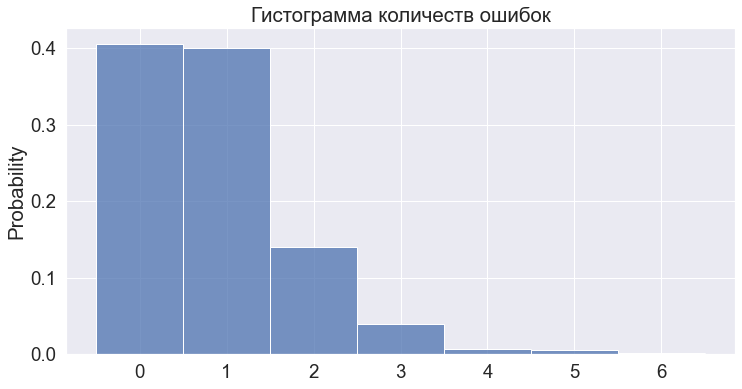
\includegraphics[width=0.8\linewidth]{hist_1}
				\label{ris:hist_1}
			\end{center}
		\end{figure}
		\framebreak
		\item Распределение ошибок по выравниваниям:
			\begin{itemize}
				\item Один к одному: 80.0\%;
				\item Один ко многим: 15.6\%;
				\item Много к одному: 4.1\%;
				\item Много ко многим: 0.2\%.
			\end{itemize}
		\framebreak		
		\item Распределение ошибок по расстоянию Дамерау-Левенштейна:
		\begin{figure}[!h]
			\begin{center}
				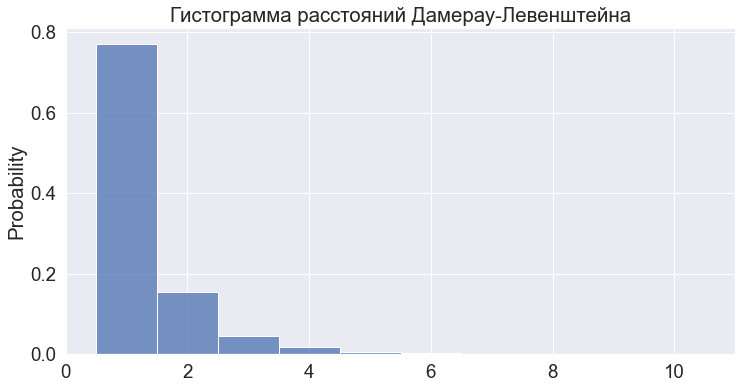
\includegraphics[width=0.8\linewidth]{hist_2}
				\label{ris:hist_1}
			\end{center}
		\end{figure}
		\item Количество исправлений, неизвестных словарю: 105.
	\end{itemize}
\end{frame}

\subsubsection{Тестовое множество}
\begin{frame}
	\frametitle{\insertsection} 
	\framesubtitle{\insertsubsection, \insertsubsubsection}
	\begin{itemize}
		\item Количество предложений: 2000;
		\item Всего исправлений: 1976.
	\end{itemize}
\end{frame}

\section{Архитектура модели}
\subsection{Алгоритм}
\begin{frame}
	\frametitle{\insertsection} 
	\framesubtitle{\insertsubsection}
		
		Предварительные действия:
		\begin{itemize}
			\item Токенизация, оформление <<черного списка>>.
			\item Генерации кандидатов и объединения токенов в группы.
		\end{itemize}
		
		Итерации исправления:
			\begin{itemize}
				\item Поиск лучшей позиции для исправления и проверка критерия останова.
				\item Исправление в выбранной позиции.
				\item Внесение позиций без исправлений в <<черный список>>.
			\end{itemize}
\end{frame}

\subsection{Candidate Generator}
\begin{frame}
	\frametitle{\insertsection} 
	\framesubtitle{\insertsubsection}
	Модель для генерации кандидатов с их признаками. 
	
	Для каждого токена генерируется список кандидатов при помощи моделей:
	\begin{itemize}
		\item \texttt{LevenshteinSearcher}  --- поиск слов из словаря на заданном расстоянии Дамерау-Левенштейна.
		\item \texttt{PhoneticSearcher} --- поиск слов из словаря с тем же фонетическим кодом.
		\item \texttt{HandcodeSearcher} --- собранная вручную таблица.
	\end{itemize}

	Используется словарь: \url{https://github.com/danakt/russian-words/}.
	
	Существует также механизм объединения токенов.
\end{frame}

\subsubsection{\texttt{LevenshteinSearcher}}
\begin{frame}
	\frametitle{\insertsection} 
	\framesubtitle{\insertsubsection, \insertsubsubsection}
	
	\begin{itemize}
		\item Реализация модели взята из библиотеки DeepPavlov: \url{https://github.com/deepmipt/DeepPavlov/tree/master/deeppavlov/models/spelling_correction/levenshtein}
		\item Словарь хранится в виде префиксного бора.
		\item Для поиска используется алгоритм $A^*$ с $h_2$-эвристикой из статьи [\textcite{Oflazer1996}].
		\item Позволяет находить ошибки ненужного слияния слов (\textit{вобщем} $\rightarrow$ \textit{в общем}).
	\end{itemize}
\end{frame}

\subsubsection{\texttt{PhoneticSearcher}}
\begin{frame}
	\frametitle{\insertsection} 
	\framesubtitle{\insertsubsection, \insertsubsubsection}
	
	\begin{itemize}
		\item Модель фонетического кодирования слов.
		\item Реализация по статье [\textcite{Sorokin2016}].
		\item Позволяет находить словарные слова похожие по звучанию: (\textit{пользовацца} $\rightarrow$ \textit{пользоваться}).
		\item Позволяет исправлять ошибки с повторением гласных (\textit{дооолго} $\rightarrow$ \textit{долго}).
	\end{itemize}
\end{frame}

\subsubsection{\texttt{HandcodeSearcher}}
\begin{frame}
	\frametitle{\insertsection} 
	\framesubtitle{\insertsubsection, \insertsubsubsection}
	
	Вручную созданная таблица для предложения кандидатов.\\~\\
	
	Построение:
		\begin{enumerate}
			\item Были взяты тексты из социальных сетей, которые попали в корпус <<Тайга>>: \url{https://tatianashavrina.github.io/taiga_site/}
			\item Был взят словарь, являющийся объединением словарей Хагена и wiktionary.
			\item Несловарные слова были упорядочены по частоте встречаемости.
			\item Было проанализировано около 5000 слов, среди которых найдено около 140 исправлений.
			\item Добавлено два словарных исправления по обучающему множеству и несколько исправлений, исходя из собственного опыта.
		\end{enumerate}
\end{frame}

\subsubsection{Генерация признаков}
\begin{frame}
	\frametitle{\insertsection} 
	\framesubtitle{\insertsubsection, \insertsubsubsection}
	
	Помимо нахождения самих кандидатов для них также вычисляются признаки:
	\begin{itemize}
		\item Признаки позиции.
		\item Признаки источника.
		\item Индикатор текущего кандидата.
		\item Индикатор оригинального кандидата.
		\item Содержание пробелов/дефисов.
		\item Индикатор словарности (актуально только для оригинального токена).
		\item Индикатор объединения.
	\end{itemize}
\end{frame}

\subsubsection{Объединение токенов}
\begin{frame}
	\frametitle{\insertsection} 
	\framesubtitle{\insertsubsection, \insertsubsubsection}
	В модели генерации кандидатов есть механизм для объединения двух последовательно идущих токенов в один для их совместного рассмотрения. \\~\\
	
	Это нужно для того, чтобы уметь исправлять вставки лишних пробелов: (\textit{и так} $\rightarrow$ \textit{итак}), (\textit{как то} $\rightarrow$ \textit{как-то}). \\~\\
	
	Алгоритм заключается в последовательном просмотре токенов слева направо и их жадном объединении если получаем словарное слово убрав пробел или заменив его на дефис.
	
\end{frame}

\subsection{Position Selector}
\begin{frame}
	\frametitle{\insertsection} 
	\framesubtitle{\insertsubsection}
	Модель для нахождения позиции исправления на текущей итерации и проверки критерия останова. В ее основе лежит использование языковых моделей слева-направо и справа-налево.
\end{frame}

\subsubsection{Алгоритм работы}
\begin{frame}
	\frametitle{\insertsection} 
	\framesubtitle{\insertsubsection, \insertsubsubsection}
	Алгоритм работы:
	\begin{itemize}
		\item  Для каждой позиции и каждого кандидата находится логарифм вероятности от этих моделей.
		\item Считается агрегирующая метрика --- среднее гармоническое логарифмов вероятностей от левой и правой моделей. Для каждой позиции находится разница этой метрики между лучшим кандидатом и текущим.
		\item В качестве позиции для исправления позиция берется позиция, которая
		\begin{itemize}
			\item не находится в <<черном списке>>,
			\item разница метрик в которой максимальна и превышает некий порог.
		\end{itemize}
		\item Вычисленные вероятности и метрика записываются в признаки кандидатов.
	\end{itemize}
\end{frame}

\subsubsection{Языковые модели}
\begin{frame}
	\frametitle{\insertsection} 
	\framesubtitle{\insertsubsection, \insertsubsubsection}
	Для построения языковых моделей была взята библиотека KenLM. 
	\begin{itemize}
		\item В качестве обучающих данных была взята часть корпуса <<Тайга>>.
		\item Текст был переведен в нижний регистр, из него была удалена пунктуация.
		\item Были обучены 3-граммные модели, использующие модифицированное сглаживание Кнезера-Нея: [\textcite{Chen1996}].
	\end{itemize}
\end{frame}

\subsubsection{Supervised модель}
\begin{frame}
	\frametitle{\insertsection} 
	\framesubtitle{\insertsubsection, \insertsubsubsection}
	Была предпринята попытка обучить supervised модель на основе признаков кандидатов. \\~\\
	
	Хоть модель и имела большую полноту при нахождении позиций с ошибками это не привело к улучшению результата.\\~\\
	
	По всей видимости, модель хоть и находила новые позиции с ошибками, но подходящих кандидатов для их исправления не было.
\end{frame}

\subsection{Candidate Scorer}
\begin{frame}
	\frametitle{\insertsection} 
	\framesubtitle{\insertsubsection}
	Модель ранжирования кандидатов на основе BERT [\textcite{Devlin2019}] и других признаков.
\end{frame}

\subsubsection{\texttt{BertScorer}}
\begin{frame}
	\frametitle{\insertsection} 
	\framesubtitle{\insertsubsection, \insertsubsubsection}
	Ранжирование на основе предсказания замаскированных токенов при помощи модели. Используется Conversational RuBERT.\\~\\
	
	Алгоритм:
	\begin{itemize}
		\item Токенизация предложений при помощи WordPiece-токенизатора, использующегося в BERT.
		\item Токенизация кандидатов.
		\item Для каждого подтокена в кандидате измерить логарифм его вероятности, отключив механизм внимания для других подтокенов.
		\item Все полученные логарифмы вероятностей для одного кандидата усреднить.
	\end{itemize}
\end{frame}

\subsubsection{Supervised модель}
\begin{frame}
	\frametitle{\insertsection} 
	\framesubtitle{\insertsubsection, \insertsubsubsection}
	\begin{itemize}
		\item Было выяснено, что ранжирование только при помощи BERT имеет весьма низкое качество, ему не хватает модели ошибок.
		\item Протестировав модель на обучающем множестве, удалось собрать выборку, где было известно какие кандидаты и с какими признаками попадают в Candidate Scorer.
		\item В качестве supervised моделей были испытаны модели: ranking SVM, CatBoost.
		\item Признаки:
		\begin{itemize}
			\item признаки из candidate generator,
			\item признаки из position selector,
			\item признаки BERT:
			\begin{itemize}
				\item среднее логарифов вероятностей подтокенов,
				\item сумма логарифмов вероятностей подтокенов,
				\item количество подтокенов.
			\end{itemize}
		\end{itemize}
	\end{itemize}
\end{frame}

\section{Результаты}
\subsection{Напоминание целевых метрик}
\begin{frame}
	\frametitle{\insertsection} 
	\framesubtitle{\insertsubsection}
		Пусть имеется текст из $n$ предложений, тогда обозначим $g_i$ -- множество корректных исправлений предложения $i$, а $e_i$ -- множество наших исправлений. 
		\begin{gather*}
			R = \frac{\sum_{i=1}^n |g_i \cap e_i|}{\sum_{i=1}^n |g_i|},
			\\
			P = \frac{\sum_{i=1}^n |g_i \cap e_i|}{\sum_{i=1}^n |e_i|}.
		\end{gather*}
		Целевая метрика:
		\begin{equation*}
			F_1 = \frac{2 P R}{P + R}.
		\end{equation*}
			
\end{frame}

\subsection{Сравнение с другими моделями}
\begin{frame}
	\frametitle{\insertsection} 
	\framesubtitle{\insertsubsection}
		\begin{table}
		\begin{center}
			\small
			\begin{tabular}{c|c|c|c}
				\hline
				\textbf{Spell Checker} & \textbf{Precision}  & \textbf{Recall} & $\boldsymbol{F_1}$  \\
				\hline
				Yandex.Speller & 83.09  & 59.86 & 69.59  \\
				JamSpell & 44.57 & 35.69 & 39.64 \\
				SpellRuEval Baseline & 55.91 & 46.41 & 50.72  \\
				SpellRuEval Winner & 81.98 & 69.25 & 75.07  \\
				Лучшая модель & \textbf{86.56} & \textbf{72.37} & \textbf{78.83} \\
				Быстрая модель & 85.30 & 70.80 & 77.38 \\
				\hline
			\end{tabular}
		\end{center}
		\caption{Сравнение результатов различных моделей.}
	\end{table}
\end{frame}

\subsection{Сравнение различных вариантов модели}
\begin{frame}
	\frametitle{\insertsection} 
	\framesubtitle{\insertsubsection}
	\begin{table}
		\begin{center}
			\small
			\begin{tabular}{c|c|c|c}
				\hline
				\textbf{Spell Checker} & \textbf{Precision}  & \textbf{Recall} & $\boldsymbol{F_1}$  \\
				\hline
				BERT & 47.16 & 55.82 & 51.12 \\
				SVM & 84.86  & 66.95 & 74.85  \\
				SVM+comb. & 84.67  & 69.59 & 76.39  \\
				SVM+BERT & 86.35  & 69.48 & 77.01  \\
				SVM+BERT+comb. & 86.35 & \textbf{72.37} & 78.74 \\
				CatBoost & 85.42  & 67.61 & 75.48  \\
				CatBoost+comb. & 85.30  & 70.80 & 77.38  \\
				CatBoost+BERT & \textbf{87.08}  & 69.59 & 77.36  \\
				CatBoost+BERT+comb. & 86.56 & \textbf{72.37} & \textbf{78.83} \\
				\hline
			\end{tabular}
		\end{center}
		\caption{Сравнение результатов вариаций модели.}
	\end{table}
\end{frame}

\subsection{Скорость работы}
\begin{frame}
	\frametitle{\insertsection} 
	\framesubtitle{\insertsubsection}
	Лучшая модель: $\approx$ 0.6 предл./с. 
	\begin{itemize}
		\item Candidate Generator: 5.3\%;
		\item Position Selector: 9.7\%;
		\item Candidate Scorer: 84.9\%.
	\end{itemize}
	
	Быстрая модель: $\approx$ 4.8 предл./с.
	\begin{itemize}
		\item Candidate Generator: 43.8\%;
		\item Position Selector: 50.4\%;
		\item Candidate Scorer: 5.4\%.
	\end{itemize}
\end{frame}

\section{Планы работ}
\begin{frame}
	\frametitle{\insertsection} 
	\framesubtitle{\insertsubsection}
	\begin{enumerate}
		\item Провести испытания с новым словарем.
		\item Поэкспериментировать над некоторыми гиперпараметрами:
			\begin{itemize}
				\item вариация BERT;
				\item вариация языковых моделей;
				\item размер вручную заданной таблицы.
			\end{itemize}
		\item Писать текст диплома.
	\end{enumerate}
\end{frame}

\section{Заключение}
\begin{frame}
	\frametitle{\insertsection} 
	Спасибо за внимание!\\~\\
	
	Исходники доступны по ссылке: \url{https://github.com/Mr-Geekman/bd-research}.
\end{frame}

\section{Литература}
\begin{frame}[allowframebreaks]{reference}
	\frametitle{\insertsection} 
	\printbibliography
\end{frame}

\end{document}